\documentclass[12pt, a4paper, twoside, openany, titlepage]{book}

% Inclusion of packages:

% The geometry package is used to alter the margins of each page
\usepackage[inner=5cm,outer=2cm,ignoreheadfoot,top=4cm,bottom=5cm,footskip=4cm]{geometry}
% the url package is used ot include URLs without messing up the rest
% of the latex
\usepackage[hyphens]{url}
% the graphicx package lets me include figures
\usepackage{graphicx}
% the listings package lets me include program listings
\usepackage{listings}
% the caption package lets me specify float caption properties
\usepackage[]{caption}
% the color package lets me define colors as strings
\usepackage{color}
% the url package lets me include urls
\usepackage{url}
% use package upquote to make all verbatim quotes straight quotes
\usepackage{upquote}
% the needspace package helps to keep command line block together
\usepackage{needspace}
%
\usepackage[hang,flushmargin,multiple,perpage]{footmisc}
%
\usepackage{fancyhdr}
% use package makeidx to create an index
\usepackage{makeidx}
% use package nameref to be able to refer to sections by name
\usepackage{nameref}

\makeindex

% Additional configuration:
\setlength{\captionmargin}{2.5cm}
\setlength{\parindent}{0pt}
\setlength{\parskip}{0.75em}
\setlength{\skip\footins}{2cm}

% define a bunch of color strings
\definecolor{gray}{rgb}{0.5,0.5,0.5}
\definecolor{lgray}{rgb}{0.9,0.9,0.9}
\definecolor{darkgray}{rgb}{0.15,0.15,0.15}
\definecolor{black}{rgb}{0,0,0}
\definecolor{white}{rgb}{1,1,1}

\lstdefinestyle{basic}{basicstyle=\scriptsize\ttfamily,
   numbersep=3mm,
   tabsize=4,
   showspaces=false,
   showstringspaces=false,
   frame=none,
   framexleftmargin=0mm,
   framexrightmargin=0mm,
   aboveskip = 0.5em,
   belowskip = -0.5em,
   xleftmargin = 0mm,
   breaklines = false,
}
\lstdefinestyle{bash}{basicstyle=\color{black}\scriptsize\ttfamily,
                      language=bash,
                      keywords={},
                      keywordstyle=\color{black},
                      commentstyle=\color{black},
                      stringstyle=\color{black},
                      backgroundcolor=\color{lgray}
}
\lstdefinestyle{Java}{basicstyle=\color{black}\scriptsize\ttfamily,
                      language=Java,
                      backgroundcolor=\color{lgray}
}


\newcommand{\mytilde}{\raise.17ex\hbox{$\scriptstyle\sim$}}


\fancypagestyle{plain}{%
\fancyhf{} % clear all header and footer fields
\renewcommand{\headrulewidth}{0pt}
\renewcommand{\headrulewidth}{0pt}
\fancyfoot[OC,EC]{--\ \thepage{}\ --}
}%fancypagestyle


\renewcommand{\captionfont}{\footnotesize}
\renewcommand{\captionlabelfont}{\sffamily}


\newcommand{\insertemptypage}[0]{
\vfill
\newpage
\thispagestyle{empty}
\mbox{}
\pagebreak
}



\author{Jurriaan H. Spaaks}

\title{\textbf{Distributed Computing with Xenon} \\ tutorial}

\hyphenation{compiled Sun/Oracle JRE JDK sourceSet sub-directory examples button}








\begin{document}

\frontmatter

\maketitle

\insertemptypage{}

\pagestyle{plain}


\tableofcontents
\insertemptypage{}

\mainmatter












\chapter{Introduction}

Many scientific applications require far more computation or data storage than can be handled on a regular PC or laptop. For such applications, access to remote storage and compute facilities is essential. Unfortunately, there is not a single standardized way to access such facilities. There are many competing protocols and tools in use by the various scientific data centers and commercial online providers.

As a result, application developers are forced to either select a few protocols they wish to support, thereby limiting which remote resources their application can use, or implement support for all of them, leading to excessive development time.

Xenon is a library designed to solve this problem. It offers a simple, unified programming interface to many remote computation and data storage facilities, and hides the complicated protocol and tool specific details from the application.

Xenon consists of three pillars: \textit{credentials}\index{Xenon!pillars!credentials}, \textit{files}\index{Xenon!pillars!files}, and \textit{jobs}\index{Xenon!pillars!jobs} (Figure~\ref{fig:xenon-design}).
%
The credentials pillar contains functionality pertaining to gaining access to (remote) systems, for example by using passwords, public/private keys, certificates, etc.
%
The files pillar contains all functionality relating to the filesystem: creation, deletion, and copying of files and directories, checking if a file or directory exists, listing directory contents, etc.
%
Lastly, the jobs pillar contains functionality relating to jobs, such as submitting and cancelling a job, checking a job's status (\textit{polling}\index{polling}), etc.

\begin{figure}[ht]
\centering
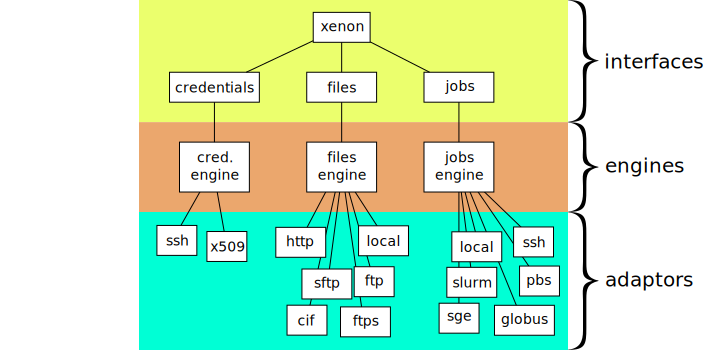
\includegraphics[width=1.0\columnwidth]{images/xenon-design}
\caption{\label{fig:xenon-design} Xenon is built on 3 pillars: credentials\index{Xenon!pillars!credentials}, files\index{Xenon!pillars!files} and jobs\index{Xenon!pillars!jobs}. Each pillar consists of an interface\index{Xenon!interface}, an engine\index{Xenon!engine}, and multiple adaptors\index{Xenon!adaptor}.}
\end{figure}

% TODO issue #23 examples of what you can do with it

\section{Purpose of this document}

This document aims to help users without much prior knowledge about Java programming and without much experience in using remote systems to understand the basics of how to use the Xenon library. At the end of the tutorial you should have enough information to be able to start exploring on your own.

\section{Version information}

It is assumed that you are using one of the Ubuntu-based operating systems (I'm using Linux Lubuntu 14.04.3 LTS). Nonetheless, most of the material covered in this manual should be usable on other Linux distributions with minor changes. The manual is written to be consistent with Xenon release 1.1.0\footnote{For releases, see \url{https://github.com/NLeSC/Xenon/releases}}.






\chapter{Basic usage}

\needspace{6\baselineskip}
To use a minimal feature set of the Xenon library, you'll need the following software packages:
\begin{enumerate}
\item{\textit{Git}\index{Git}, a version management system;}
\item{\textit{Java}\index{Java}, a general purpose programming language;}
\end{enumerate}


The following sections describe the necessary steps in more detail.




\section{Installing Git}
\index{Installing Git}

Open a terminal (default keybinding Ctrl + Alt + t). The shell should be Bash\index{Bash}. You can check this with:
\Needspace{5\baselineskip}
\begin{lstlisting}[style=basic,style=bash]
echo $0
\end{lstlisting} % fix syntax highlighting by inserting an extra dollar sign $
which should return \texttt{/bin/bash}.


\Needspace{5\baselineskip}
Now install \texttt{git}\index{Git!git@\texttt{git}} if you don't have it already:
\begin{lstlisting}[style=basic,style=bash]
sudo apt-get install git
\end{lstlisting}

After the install completes, we need to get a copy of the examples. We will use \texttt{git} to do so. Change into the directory that you want to end up containing the top-level repository directory. I want to put the Xenon examples in my home directory, so for me that means:
\begin{lstlisting}[style=basic,style=bash]
cd ${HOME}
\end{lstlisting} % fix syntax highlighting by inserting an extra dollar sign $

\Needspace{5\baselineskip}
Then clone the Xenon-examples repository into the current directory:
\begin{lstlisting}[style=basic,style=bash]
git clone https://github.com/NLeSC/Xenon-examples.git
\end{lstlisting}
This will create a directory \texttt{\mytilde{}/Xenon-examples} that contains the source code of the Xenon examples.






\section{Installing Java}
\index{Installing Java}

Xenon is a Java library, therefore it needs Java in order to run. Java comes in different versions identified by a name and a number. The labeling is somewhat confusing\footnote{See for example \url{http://stackoverflow.com/questions/2411288/java-versioning-and-terminology-1-6-vs-6-0-openjdk-vs-sun}}. This is partly because Java was first developed by Sun Microsystems (which was later bought by Oracle Corporation), while an open-source implementation is also available (it comes standard with many Linuxes). Furthermore, there are different flavors for each version, each flavor having different capabilities. For example, if you just want to \textit{run} Java applications, you need the JRE\index{JRE} (Java Runtime Environment\index{Java Runtime Environment}); if you also want to \textit{develop} Java software, you'll need either an SDK\index{SDK} (Software Development Kit\index{Java Software Development Kit}) from Sun/Oracle, or a JDK\index{JDK} (Java Development Kit\index{Java Development Kit}) if you are using the open-source variant.

Check if you have Java and if so, what version you have:
\begin{lstlisting}[style=basic,style=bash]
java -version
\end{lstlisting}
That should produce something like:
\begin{lstlisting}[style=basic,style=bash]
java version "1.7.0_79"
OpenJDK Runtime Environment (IcedTea 2.5.6) (7u79-2.5.6-0ubuntu1.14.04.1)
OpenJDK 64-Bit Server VM (build 24.79-b02, mixed mode)
\end{lstlisting}
Note that `Java version 1.7' is often referred to as `Java 7'.

If you don't have Java yet, install it with:
\begin{lstlisting}[style=basic,style=bash]
sudo apt-get install default-jdk
\end{lstlisting}
this will install the open-source variant of Java (`OpenJDK'\index{Java!OpenJDK}\index{OpenJDK}).






\section{Building with \texttt{gradlew}}

To check if everything works, we first need to build the example from source and then run the example from the command line.

At this point, \mytilde/\url{Xenon-examples} only contains files directly related to the source code of the example files. However, in order to build and run the examples successfully, we'll need a few more things. Naturally, we'll need a copy of the Xenon library, but the Xenon library in turn also has dependencies that need to be resolved. Because the process of fitting together the right libraries is quite a lot of work, we have automated it. For this, we use the build automation tool\index{build automation}\index{build tool} Gradle\index{Gradle}\footnote{\url{http://gradle.org/}}. Interestingly, you do not need to install Gradle for it to work (although you do need Java). This is because the Xenon-examples repository already includes a script called \texttt{gradlew}, which will download a predefined version of the Gradle program upon execution. The advantage of using \texttt{gradlew} for this is that the resulting build setup will be exactly the same as what the developers use, thus avoiding any bugs that stem solely from build configuration differences.

The \texttt{gradlew} script can be run with arguments. For example, running
\begin{lstlisting}[style=basic,style=bash,escapeinside={(*@}{@*)}]
cd ${HOME}/Xenon-examples
./gradlew dependencies
\end{lstlisting} % dummy $
prints a list of the dependencies (of which there are quite many), and

\begin{lstlisting}[style=basic,style=bash,escapeinside={(*@}{@*)}]
./gradlew clean
\end{lstlisting} % dummy $
cleans up the files pertaining to any previous builds.

\texttt{dependencies} and \texttt{clean} are referred to as `Gradle tasks', `build tasks' or just `tasks'\index{Gradle!tasks}. Tasks are defined in a so-called build file\index{Gradle!build file} called \url{build.gradle}. To get an overview of all available tasks you could read through \url{build.gradle}, or you could simply run:
\begin{lstlisting}[style=basic,style=bash,escapeinside={(*@}{@*)}]
./gradlew tasks
\end{lstlisting} % dummy $

or

\begin{lstlisting}[style=basic,style=bash,escapeinside={(*@}{@*)}]
./gradlew tasks --all
\end{lstlisting} % dummy $

If you run \texttt{./gradlew tasks}, you'll see a line at the top that says that the default task is called \texttt{shadowJar}\index{shadowJar@\texttt{shadowJar}}\footnote{\url{https://github.com/johnrengelman/shadow}}. \texttt{shadowJar} bundles any and all dependencies into one large jar, sometimes referred to as a `fat jar'\index{fat jar}. Once you figure out what to put in it, using a fat jar makes deployment more robust against forgotten-dependency errors. Lucky for you, someone has already figured out how to make the fat jar, and has even written it down in a file that Gradle can understand.

Run \texttt{./gradlew} (without any arguments) to start the default task. The following things will happen:
\begin{enumerate}
\item{the correct version of Gradle will be downloaded;}
\item{the Xenon library will be downloaded;}
\item{any dependencies that the Xenon library has will be downloaded;}
\item{all of that will then be compiled;}
\item{a fat jar will be created.}
\end{enumerate}



\section{Running an example}

So at this point we have compiled the necessary Java classes; now we need to figure out how to run them.

The general syntax for running compiled Java programs from the command line\index{Java!from the command line} is as follows:
\begin{lstlisting}[style=basic,style=bash,escapeinside={(*@}{@*)}]
java (*@\textit{<fully qualified classname>}@*)
\end{lstlisting}
We will use the \texttt{DirectoryListing} example from the \url{nl.esciencecenter.xenon.examples.files} package. As the name implies, it lists the directory contents of a given directory. The fully qualified classname for our example is \url{nl.esciencecenter.xenon.examples.files.DirectoryListing}, but if you try to run
\begin{lstlisting}[style=basic,style=bash,escapeinside={(*@}{@*)}]
cd ${HOME}/Xenon-examples
java nl.esciencecenter.xenon.examples.files.DirectoryListing
\end{lstlisting} % dummy $
you will get the error below:
\begin{lstlisting}[style=basic,style=bash,escapeinside={(*@}{@*)}]
Error: Could not find or load main class \
nl.esciencecenter.xenon.examples.files.DirectoryListing
\end{lstlisting}

This is because the \url{java} executable tries to locate our class \url{nl.esciencecenter.xenon.examples.files.DirectoryListing}, but we haven't told \url{java} where to look for it. We can resolve that by specifying a list of one or more directories using \texttt{java}'s classpath option \texttt{-cp}\index{Java!from the command line!classpath}\index{Java!from the command line!-cp@\texttt{-cp}}.

Directory names can be passed to \texttt{java} as a colon-separated list, in which directory names can be relative to the current directory. Furthermore, the syntax is slightly different depending on what type of file you want \texttt{java} to find in a given directory: if you want \texttt{java} to find compiled Java classes, use the directory name; if you want \texttt{java} to find jar files, use the directory name followed by the name of the jar (or use the wildcard \texttt{*} if you want \texttt{java} to find any jar from a given directory). Finally, the order within the classpath is significant.\index{Java!classpath}


We want Java to find the fat jar \url{Xenon-examples-all.jar} from \url{build/libs}. Using paths relative to \mytilde\url{/Xenon-examples}, our classpath thus becomes \url{build/libs/Xenon-examples-all.jar}. However, if we now try to run
\begin{lstlisting}[style=basic,style=bash,escapeinside={(*@}{@*)}]
cd ${HOME}/Xenon-examples
java -cp 'build/libs/Xenon-examples-all.jar' \
nl.esciencecenter.xenon.examples.files.DirectoryListing
\end{lstlisting}
% dummy $
it still does not work yet, because \url{DirectoryListing} takes exactly one input argument that defines the location (URI\index{URI}) of the directory whose contents we want to list. URIs generally consist of a \textit{scheme}\index{URI!scheme} followed by the colon character~\texttt{:}, followed by a \textit{path}\index{URI!path}\footnote{The full specification of a URI is (optional parts in brackets): \\ \texttt{scheme:[//[user:password@]domain[:port]][/]path[?query][#fragment]}\label{footnote:format-uri}}. For a local file, the scheme name is \texttt{local}. The path is the name of the directory we want to list the contents of, such as \texttt{\$\{PWD\}} (the present working directory).

Putting all that together, we get:

\begin{lstlisting}[style=basic,style=bash,escapeinside={(*@}{@*)}]
cd ${HOME}/Xenon-examples
java -cp 'build/libs/Xenon-examples-all.jar' \
nl.esciencecenter.xenon.examples.files.DirectoryListing local:${PWD}
\end{lstlisting} \label{snip:directory-listing-local}

If all goes well, you should now see the contents of the current directory as an INFO message.


\section{Setting the log level}
\label{sec:setting-the-log-level-command-line}

Xenon uses the logback\footnote{\url{http://logback.qos.ch/}}\index{logback library}\index{logger} library for much of the output. For this, developers have sprinkled the code with so-called \textit{logger}\index{logger} statements that produce messages. Each message has been annotated as an error, a warning, debugging information, or as a plain informational message. The logback library lets the user configure where each type of message should be routed. For example, warnings and informational messages may be routed to standard output, while error messages may be routed to standard error. Furthermore, it gives the user control of how each message should be formatted, for example with regard to what class produced the message, and at what line exactly. The behavior of the logger can be configured by means of a file called \url{logback.xml}\index{logback.xml@\texttt{logback.xml}}. It is located at \url{src/main/resources/}. There should not be any need for you to change \url{logback.xml} too much, but if you do, make sure to re-run \texttt{./gradlew} for your changes to take effect.

By default, \url{logback.xml} uses a logging level of \texttt{INFO}, which means that warnings, errors, and informational messages are routed to standard output, but debug messages are not visible. At some point, you may find yourself in a situation where you want to change the logging level. There's two ways you can do that: first you can change the default behavior by editing the \texttt{loglevel} line in \url{src/main/resources/logback.xml}, saving it, and re-running \texttt{./gradlew}.

\Needspace{20\baselineskip}
Secondly, you can keep the defaults as they are, but only run a specific call with altered \texttt{loglevel} settings, by using command line parameters to the \texttt{java} program\index{Java!command line parameters}. For example, you could lower the logging level from \texttt{INFO} to \texttt{DEBUG} as follows:

\begin{lstlisting}[style=basic,style=bash,escapeinside={(*@}{@*)}]
cd ${HOME}/Xenon-examples
java -Dloglevel=DEBUG -cp 'build/libs/Xenon-examples-all.jar' \
nl.esciencecenter.xenon.examples.files.DirectoryListing local:${PWD}
\end{lstlisting} % dummy $

Standard output will now include messages of the \texttt{WARN}, \texttt{ERROR}, \texttt{INFO}, and \texttt{DEBUG} level, e.g.:
\begin{lstlisting}[style=basic,style=bash,escapeinside={(*@}{@*)}]
time   : 11:49:58.473 (+315 ms)
thread : main
level  : DEBUG
class  : nl.esciencecenter.xenon.examples.files.DirectoryListing:74
message: Creating a new Path...

time   : 11:49:58.473 (+315 ms)
thread : main
level  : DEBUG
class  : nl.esciencecenter.xenon.examples.files.DirectoryListing:78
message: Getting the directory attributes...

time   : 11:49:58.481 (+323 ms)
thread : main
level  : INFO
class  : nl.esciencecenter.xenon.examples.files.DirectoryListing:95
message: Directory local:/home/daisycutter/Xenon-examples exists
         and contains the following:
         .travis-ssh.sh
         run-examples.sh
         .gitignore
         doc
         build
         bin
                             (*@\textit{<some content omitted>}@*)
\end{lstlisting}



\section{Xenon's SSH adaptor}

Up till now, you've used Xenon to perform tasks on your own system (by means of Xenon's \texttt{local} adaptor\index{Xenon!adaptor!local@\texttt{local}}). Usually though, you'll want to use Xenon to perform tasks on remote systems, such as the Amazon cloud, the Lisa cluster computer, the Cartesius supercomputer, or perhaps just a single machine (but not your own). To do so, you first need to connect to them. You can use Xenon's SSH adaptor\index{Xenon!adaptor!SSH} to do so. The SSH adaptor works in a similar way as the so-called \textit{secure shell}\index{secure shell} program \texttt{ssh}\index{ssh@\texttt{ssh}} on the Linux command line. Through SSH, you can connect to a remote system and do all the things a user is allowed to do on that system (which in turn is defined by the remote system's administrator).

To keep things simple, we'll first set up an SSH connection to \url{localhost}, thus effectively connecting ourselves with ourselves. Later on in this document we'll also look at using SSH to connect to a remote system (see Section~\ref{sec:live-systems}:~\textit{\nameref{sec:live-systems}}). Additionally, we'll set up Docker to run virtual remote systems on your local machine. That way, you can emulate the behavior of one or more remote machines (see Section~\ref{sec:docker}:~\textit{\nameref{sec:docker}}) without the need for any additional hardware besides your own machine. Anyway, that's all for later---let's get started on setting up SSH to \url{localhost} first.

\subsection{\texttt{ssh} to \url{localhost}}

SSH uses the server-client model. Normally, your system is the client, while the remote system is the server. Since we will connect to \url{localhost} however, your system will play the part of both client and server.

The client needs to have a so-called \textit{public-private key pair}\index{public-private key pair}. The key pair can be generated according to different algorithms:
\texttt{dsa}\index{ssh-keygen@\texttt{ssh-keygen}!dsa@\texttt{dsa}},
\texttt{ecdsa}\index{ssh-keygen@\texttt{ssh-keygen}!ecdsa@\texttt{ecdsa}},
\texttt{ed25519}\index{ssh-keygen@\texttt{ssh-keygen}!ed25519@\texttt{ed25519}}, or
\texttt{rsa}\index{ssh-keygen@\texttt{ssh-keygen}!rsa@\texttt{rsa}}.
The Linux program \texttt{ssh-keygen}\index{ssh-keygen@\texttt{ssh-keygen}} implements these algorithms. We will use it to generate a public-private key pair using the \texttt{rsa} algorithm, as follows:

\begin{lstlisting}[style=basic,style=bash,escapeinside={(*@}{@*)}]
# generate key pair using rsa algorithm
ssh-keygen -t rsa
# (press enter to accept the default file location ~/.ssh/id_rsa; if it
# tells you the file already exists, you can skip creation of a new key)
# (press enter to set the passphrase to an empty string)
# (press enter to confirm setting the passphrase to an empty string)
\end{lstlisting}

You should now have a directory \mytilde/\url{.ssh} with two files in it: \url{id_rsa},  the private part of the key pair and \url{id_rsa.pub}, the public part of the key pair. Note that the contents of \url{id_rsa} should remain a secret.

That's it for the client side, but you still need to do some stuff on the server side. First, install the package \texttt{openssh-server} from the Ubuntu repositories:
\begin{lstlisting}[style=basic,style=bash,escapeinside={(*@}{@*)}]
# install a server
sudo apt-get install openssh-server
\end{lstlisting} % dummy $

The server side keeps a list \mytilde/\url{.ssh/authorized_keys} of trusted identities. You have to add the identity information from \mytilde/\url{.ssh/id_rsa.pub} to it. Linux provides an easy way of doing this, as follows:
\begin{lstlisting}[style=basic,style=bash,escapeinside={(*@}{@*)}]
# copy identity, type 'yes' when prompted
ssh-copy-id ${USER}@localhost
\end{lstlisting}\index{ssh-copy-id@\texttt{ssh-copy-id}} % dummy $

On the server side, file \mytilde/\url{.ssh/authorized_keys} should now contain the information from \mytilde/\mbox{\url{.ssh/id_rsa.pub}}.



When you did \texttt{ssh-copy-id}, SSH tried to connect the current user (whose credentials are found in \mytilde/\url{.ssh/id_rsa.pub}) to the `remote' system \url{localhost}. If that was successful, there should now be a new file \mytilde/\url{.ssh/known_hosts} on the client, that contains a list of machines that we have connected to previously; i.e. these are systems we trust.

\Needspace{10\baselineskip}
Each line in  \url{known_hosts} is formatted according to: \\
\texttt{|<flag>|<salt>=|<hostname>= <key> <value>=}, where
\begin{itemize}
\item{\texttt{<flag>} is a flag. Mine says \texttt{1} to signify that the third element \texttt{<hostname>} is hashed using the SHA1 algorithm;}
\item{\texttt{<salt>} is the (public) salt used to encrypt the host name;}
\item{\texttt{<hostname>} is the (hashed) host name;}
\item{\texttt{<key>}\texttt{<value>} pairs, e.g. the key \url{ecdsa-sha2-nistp256} and its value\\ \texttt{AAAAE2V\textit{...<characters omitted>...}RpXi/rE}, representing the public key of the `remote' system which was generated when we installed \texttt{openssh-server} and which is stored at \url{/etc/ssh/ssh_host_ecdsa_key.pub}\footnote{You can show the fingerprint of the server's public key file using:\\
\texttt{ssh-keygen -l -f /etc/ssh/ssh\_host\_ecdsa\_key.pub}\\
The number that \texttt{ssh-keygen} returns should be the same number that was displayed in your terminal when you did \texttt{ssh-copy-id \${USER}@localhost}.} on hostname.}
\end{itemize}
Xenon uses \texttt{known\_hosts} to automatically connect to a (known) remote system, without having to ask for credentials every time.

\Needspace{7\baselineskip}
For passwordless SSH to work correctly, permissions are important\index{ssh@\texttt{ssh}!permissions}. You can check the octal representation of a file's permissions by:
\begin{lstlisting}[style=basic,style=bash,escapeinside={(*@}{@*)}]
stat -c "%a" (*@\textit{<filename>@*)}
\end{lstlisting}
and you can change them with:
\begin{lstlisting}[style=basic,style=bash,escapeinside={(*@}{@*)}]
# change (*@\textit{<filename>@*)}'s permissions to rwx------ or octal 700
chmod 700 (*@\textit{<filename>@*)}
\end{lstlisting}

On the server-side, verify that permissions are set correctly on the following files and directories:
\begin{enumerate}
\item{\url{${HOME}/} and \url{${HOME}/.ssh/} should be writable only by owner, not by group or all. On my system, I have octal permission 700. }
\item{\url{${HOME}/.ssh/authorized_keys} should be writable only by owner, not by group or all. On my system, I have octal permission 600. } % dummy $
\end{enumerate}

On the client-side, verify that permissions are set correctly on the following files and directories:
\begin{enumerate}
\item{\url{${HOME}/}} and \url{${HOME}/.ssh/} should be writable only by owner, not by group or all. On my system, I have octal permission 700. }
\item{\url{${HOME}/.ssh/id_rsa} should be octal permission 600. \texttt{ssh-copy-id} should have set the permissions correctly.} % dummy $
\item{\url{${HOME}/.ssh/id_rsa.pub} should be octal permission 644. \texttt{ssh-copy-id} should have set the permissions correctly.} % dummy $
\end{enumerate}

\begin{lstlisting}[style=basic,style=bash,escapeinside={(*@}{@*)}]
# now try to log in without entering key:
ssh ${USER}@localhost
\end{lstlisting} % dummy $

If all goes well, you should be logged in automatically without having to enter a password. You can log out of the SSH session with:
\begin{lstlisting}[style=basic,style=bash,escapeinside={(*@}{@*)}]
logout
\end{lstlisting}



\section{\texttt{DirectoryListing} through SSH}

So now that we have configured passwordless SSH to \texttt{localhost}, listing the contents of a directory on \texttt{localhost} is actually pretty simple. In the URI that you pass as a command line argument to \texttt{DirectoryListing} (see page~\pageref{snip:directory-listing-local}), replace \texttt{local} by \texttt{ssh}, and supply \url{localhost} as the domain name. Also note that the inclusion of a domain makes it necessary to include \texttt{//} between \texttt{ssh} and \texttt{localhost} (see footnote on formatting URIs on page~\pageref{footnote:format-uri}). So the complete call becomes:

\begin{lstlisting}[style=basic,style=bash,escapeinside={(*@}{@*)}]
cd ${HOME}/Xenon-examples
java -cp 'build/libs/Xenon-examples-all.jar' \
nl.esciencecenter.xenon.examples.files.DirectoryListing \
ssh://localhost${PWD}
\end{lstlisting} % dummy $

If all goes well, you should see the same directory contents as before, but now viewed through SSH.

\section{Example usage of local and SSH adaptors}

\Needspace{6\baselineskip}
We have compiled a list of examples demonstrating various uses of the \texttt{local} adaptor and the \texttt{ssh} adaptor. Your system is now configured correctly to run all of them. This is most easily accomplished by starting the \texttt{run-examples.sh} script we have prepared:
\begin{lstlisting}[style=basic,style=bash,escapeinside={(*@}{@*)}]
cd ${HOME}/Xenon-examples
./run-examples.sh
\end{lstlisting} % dummy $

Note that you can edit the loglevel by changing the parameter \texttt{LOGLEVEL} in \url{run-examples.sh}.





\section{A minimal Eclipse installation}
\index{Eclipse!minimal installation}

So now that we've verified that everything works, we can start thinking about doing some development work. Let's first look at the Java editor Eclipse.

Eclipse\index{Eclipse} is a very powerful, free, open-source, integrated development environment for Java (and many other languages). It is available in most Linuxes from their respective repositories. By default, Eclipse comes with many features, such as Git (version control)\index{Git}, Mylyn (task management)\index{Mylyn}, Maven (building)\index{Maven}, Ant (building)\index{Ant}, an XML editor, as well as some other stuff. While these features are nice, they can get in the way if you're new to code development with Java using Eclipse. We will therefore set up a minimal Eclipse installation which includes only the Eclipse platform and the Java related tools (most importantly, the debugger). Feel free to skip this next part if you're already familiar with Eclipse.


Go to \url{http://download.eclipse.org/eclipse/downloads/}. Under `Latest release', click on the link with the highest version number. It will take you to a website that has a menu in the upper left corner. From that menu, select the item `Platform Runtime binary', then download the file corresponding to your platform (for me, that is \url{eclipse-platform-4.5-linux-gtk-x86_64.tar.gz}). Go back to the menu by scrolling up, then select the item `JDT Runtime binary', and download the file (there should be only one; for me that is \url{org.eclipse.jdt-4.5.zip}).

Now go to where you downloaded those two files to. Uncompress \url{eclipse-platform-4.5-linux-gtk-x86_64.tar.gz} and move the uncompressed files to a new directory \mytilde\url{/opt/minimal-eclipse/} (they can be anywhere, really, but \mytilde\url{/opt} is the conventional place to install user-space programs on Linux). Start Eclipse by running \url{eclipse} from \mytilde\url{/opt/minimal-eclipse/eclipse}.

In Eclipse's menu go to \textsf{Help}, then select \textsf{Install New Software...} . Near the bottom of the dialog, uncheck \textsf{Group items by category}. Then click the top-right button labeled \textsf{Add...} and click \textsf{Archive...} . Then navigate to the second file you downloaded, \url{org.eclipse.jdt-4.5.zip} and select it. In the dialog, a new item \textsf{Eclipse Java Development Tools} should appear. Make sure it's checked, then click \textsf{Next} and \textsf{Finish}. When Eclipse restarts, you should have everything you need for Java development, without any of the clutter!

\index{Bash!alias}
\index{Bash!alias!miniclipse@\texttt{miniclipse}}

Adding a Bash alias to \mytilde\url{/.bash_aliases} will make it easier to start the program. I've used
\begin{lstlisting}[style=basic,style=bash,escapeinside={(*@}{@*)}]
echo "alias miniclipse='${HOME}/opt/minimal-eclipse/eclipse/eclipse'" >> \
${HOME}/.bash_aliases
\end{lstlisting}
to do so (restart your terminal to use the \texttt{miniclipse} alias).

\section{Automatic project setup with \texttt{gradlew}}

\index{Eclipse!automatic project setup}
\index{Eclipse!gradle eclipse@\texttt{gradle eclipse}}
\index{Eclipse!./gradlew eclipse@\texttt{./gradlew eclipse}}
\index{Gradle!automatic Eclipse project setup}
\index{Gradle!gradle eclipse@\texttt{gradle eclipse}}
\index{Gradle!./gradlew eclipse@\texttt{./gradlew eclipse}}

Normally, when you start a new project in Eclipse, it takes you through a series of dialogs to set up the Eclipse project in terms of the directory structure, the classpath, etc. The configuration is saved to (hidden) files \url{.project}, \url{.classpath}, and \url{.settings/org.eclipse.jdt.core.prefs}. The dialogs offer some freedom in setting up the project. This flexibility is great when you're working on some project by yourself, but when there are multiple people working together, one developer may have a different project setup than the next, and so bugs are introduced. That's why we will use \texttt{gradlew} to generate a standard project setup for us:

\Needspace{5\baselineskip}
\begin{lstlisting}[style=basic,style=bash,escapeinside={(*@}{@*)}]
cd ${HOME}/Xenon-examples
./gradlew eclipse
\end{lstlisting} % dummy $

\section{Opening the Xenon examples in Eclipse}
\index{Xenon examples!in Eclipse}
\index{Eclipse!new project}

After the Eclipse files have been generated, start Eclipse by typing the Bash alias \texttt{miniclipse} at the command line. From Eclipse's menu, select \textsf{File}$\rightarrow$\textsf{Import}. In the \textsf{Select} dialog, select \textsf{Existing projects into Workspace}, then click the button labeled \textsf{Next}.

In the next dialog (\textsf{Import projects}), use the \textsf{Browse...} button to select the project's root directory, e.g. \url{/home/daisycutter/Xenon-examples}, then click \textsf{Finish}. An item \textsf{Xenon-examples} should now be visible in the \textsf{Package explorer} pane. Expand it, and navigate to \url{src/main/java/}, then double-click \textsf{DirectoryListing.java} from the \textsf{nl.esciencecenter.xenon.examples.files} package to view its code in the editor pane.




\section{Running a Java program in Eclipse}

\index{Eclipse!running a Java program}
\index{Running a Java program in Eclipse}
\index{Java!running a program in Eclipse}

So now that we have the source code open in the editor, let's see if we can run it. You can start the program in a couple different ways. For example, you can select \textsf{Run}$\rightarrow$\textsf{Run}; you can use the key binding \textsf{Ctrl+F11}, or you can press the `Play' icon in Eclipse's GUI. If you try to run the program, however, you will get the error we saw earlier at the command line (Eclipse prints the program's output to the pane labeled \textsf{Console}):
\begin{lstlisting}[style=basic,style=bash,language=java,escapeinside={(*@}{@*)}]
time   : 18:42:04.689 (+219 ms)
thread : main
level  : ERROR
class  : nl.esciencecenter.xenon.examples.files.DirectoryListing:51
message: Example requires a URI as parameter!
\end{lstlisting}

So somehow we have to tell Eclipse about the URI (including both its scheme and its path) that we want to use to get to the contents of a directory of our chosing. You can do this through so-called \textit{Run configurations}\index{Eclipse!run configuration}. You can make a new run configuration by selecting \textsf{Run} from the Eclipse menu, then \textsf{Run configurations...}. In the left pane of the dialog that pops up, select \textsf{Java Application}, then press the \textsf{New launch configuration} button in the top left of the dialog. A new run configuration item should now become visible under \textsf{Java Application}. By default, the name of the run configuration will be the name of the class, but you can change the name to whatever you like. When you select the \textsf{DirectoryListing} run configuration in the left pane, the right pane changes to show the details of the run configuration. The information is divided over a few tabs. Select the tab labeled \textsf{Arguments}. You should see a field named \textsf{Program arguments} where you can provide the arguments that you would normally pass through the command line. Earlier, we passed the string \texttt{local:\$\{PWD\}}, but that won't work here, since \texttt{\$\{PWD\}} is a Bash environment variable, and thus not directly available from within Eclipse. Eclipse does provide a workaround for this by way of the \texttt{env\_var} variable. \texttt{env\_var} takes exactly one argument, namely the name of an environment variable, such as \texttt{PWD}. The correct text to enter into \textsf{Program arguments} thus becomes \texttt{local:\$\{env\_var:PWD\}}. Note that \texttt{\$\{env\_var:PWD\}} refers to the directory that Eclipse was started from.





\section{Debugging a Java program in Eclipse}

\index{Eclipse!debugging a Java program}
\index{Debugging a program in Eclipse}
\index{Java!debugging in Eclipse}



In my opinion, one of the most helpful features of the Eclipse interface is the debugging/inspecting variables capability. This lets you run your program line-by-line. To start debugging, you have to set a breakpoint first. Program execution will halt at this point, such that you can inspect what value each variable has at that point in your program. Setting a breakpoint is most easily accomplished by double-clicking the left margin of the editor; a blue dot will appear. Alternatively, you can press \textsf{Ctrl+Shift+b} to set a breakpoint at the current line.

Set a breakpoint at the line
\begin{lstlisting}[style=basic,style=bash,language=java,escapeinside={(*@}{@*)}]
URI uri = new URI(args[0]);
\end{lstlisting}

Now we need to set the \textit{debug configuration}\index{Eclipse!debug configuration} in a similar manner as we did for the run configuration. Select \textsf{Run} from the menu, select \textsf{Debug configurations...} (not \textsf{Run configurations...}), then select the configuration we used previously.

Run the program up to the position of the breakpoint. There are various ways to start a debug run: e.g. by selecting \textsf{Run}$\rightarrow$\textsf{Debug}; or by pressing \textsf{F11}.

You can add all kinds of helpful tools to the Eclipse window; for an overview of your options, click the \textsf{Window} menu item, then select \textsf{Show view}, then select \textsf{Other...}. Select whatever tools you like, but make sure to select the \textsf{Variables} tool from \textsf{Debug}. This tool allows you to view information about your variables while you're debugging. Use drag and drop to lay out the Eclipse window to suit your needs. Eclipse refers to its window layout as a \textit{perspective}\index{Eclipse!perspective}; perspectives can be saved by subsequently selecting \textsf{Window}, \textsf{Perspective}, and \textsf{Save perspective as...}. This allows you to have custom perspectives for development in different languages (Java, Python, C, etc.), or for different screen setups (laptop screen v. side-by-side 1920x1080 for example), or for different tasks (Java development v. Java debugging for example).

Getting back to \textsf{DirectoryListing}, execution has been halted just before the line \texttt{URI uri = new URI(args[0]);} was executed. If you now look in the \textsf{Variables} tool pane, there should be only one variable visible: \texttt{args}, which contains the string we supplied through the \textsf{Program arguments} of the debug configuration.

Press \textsf{F6} to evaluate the line. You'll see a new variable \texttt{uri} of type \texttt{URI} appear in the \textsf{Variables} pane. Expand the object to inspect it in more detail.

When you're done inspecting, press \textsf{F8} to make Eclipse evaluate your program, either up to the next breakpoint, or if there are no breakpoints, up to the end your program.

Finally, you can terminate a debug run by pressing \textsf{Ctrl+F2}. Table~\ref{tab:key-bindings-eclipse} summarizes some of the most common Eclipse key bindings used in running and debugging Java programs.


\begin{table}[!ht]
\vspace{1.0em}
\caption{Default key bindings used for running and debugging Java programs in Eclipse.\label{tab:key-bindings-eclipse}\index{Eclipse!key bindings}}
\begin{tabular}{lp{10cm}}
\vspace{0.5em}
\textbf{Default key binding} & \textbf{Description}                  \\
\textsf{F5}                  & Step in                               \\
\textsf{F6}                  & Step over                             \\
\textsf{F7}                  & Step return                           \\
\textsf{F8}                  & Continue to the next breakpoint       \\
\textsf{F11}                 & Start a debug run                     \\
\textsf{Ctrl+F2}             & Terminate a debug run                 \\
\textsf{Ctrl+Shift+b}        & Set a breakpoint at the current line  \\
\textsf{Ctrl+F11}            & Start a (non-debug) run               \\
\end{tabular}
\end{table}

\section{Setting the log level}

Earlier, we looked at how to pass custom \texttt{loglevel} values to \texttt{java} using command line parameters such as \texttt{-Dloglevel=DEBUG} (see section \ref{sec:setting-the-log-level-command-line}). Passing command line parameters is also possible in Eclipse, by altering the debug configuration (or run configuration) as follows. In Eclipse's menu, go to \textsf{Run} and select either \textsf{Run configurations...} or \textsf{Debug configurations...} as appropriate. Then, in the left pane, select the Java application whose configuration you want to adapt. In the right-hand pane, subsequently select the tab labeled \textsf{Arguments}. The second text field from the top should be labeled \textsf{VM~arguments}\index{Eclipse!VM arguments}. Here you can add command line parameters to the java program, such as \texttt{-Dloglevel=DEBUG}.






\section{Live systems}
\label{sec:live-systems}

Earlier, we set up passwordless SSH to connect to \url{localhost}. Obviously, using SSH to connect to your own system is a bit silly. Normally, you'll want to connect to a physically remote system. In the next two sections, I'll explain how to connect to SURFsara's cluster computer, Lisa, and VU University's DAS-4 cluster, respectively. If you want to follow along, you need to make sure you have an account on at least one of these systems. Check their respective websites\footnote{\url{https://userinfo.surfsara.nl/systems/lisa}}\footnote{\url{http://www.cs.vu.nl/das4/}} to see how you can apply for an account.

If for some reason you can not or do not want to connect to these systems, make sure to check Section~\ref{sec:docker}:~\textit{\nameref{sec:docker}} to learn about using virtual remote systems.

\subsection{\texttt{ssh} to SURFsara's Lisa cluster computer}

Cluster computers typically have a dedicated machine (the so-called `headnode') that serves as the main entry point when connecting from outside the cluster. For Lisa, the headnode is located at \url{lisa.surfsara.nl}.

First, I verify that I can connect to Lisa's head node, using the \texttt{ssh} command below:
\begin{lstlisting}[style=basic,style=bash,escapeinside={(*@}{@*)}]
# (my account on Lisa is called jspaaks)
ssh jspaaks@lisa.surfsara.nl
\end{lstlisting}

\Needspace{6\baselineskip}
If this is the first time you connect to the remote machine, it will generally ask if you want to add the remote machine to the list of known hosts. For example, here's what the Lisa system tells me when I try to \texttt{ssh} to it:
\begin{lstlisting}[style=basic,style=bash,escapeinside={(*@}{@*)}]
The authenticity of host 'lisa.surfsara.nl (145.100.29.210)' can't be
established.
RSA key fingerprint is b0:69:85:a5:21:d6:43:40:bc:6c:da:e3:a2:cc:b5:8b.
Are you sure you want to continue connecting (yes/no)?
\end{lstlisting}
\Needspace{6\baselineskip}
If I then type \texttt{yes}, it says\footnote{SURFsara publish RSA public key fingerprints for their systems at \url{https://userinfo.surfsara.nl/systems/shared/ssh}. The number posted there should be the same as what you have in your terminal.}:
\begin{lstlisting}[style=basic,style=bash,escapeinside={(*@}{@*)}]
Warning: Permanently added 'lisa.surfsara.nl,145.100.29.210' (RSA) to
         the list of known hosts.

                             (*@\textit{<some content omitted>}@*)
\end{lstlisting}
and asks for my password.

The result of this connection is that \mytilde\url{/.ssh/known_hosts} now includes a line for the Lisa system.

In Eclipse, go to \texttt{DirectoryListing}'s \textsf{Debug configurations} like you did before and bring up the \textsf{Arguments} tab. Instead of connecting to \url{localhost}, we now want to connect to the Lisa cluster's head node at \url{lisa.surfsara.nl}. The full URI\footnote{see page~\pageref{footnote:format-uri} for URI's format specification} should now be \url{ssh://jspaaks@lisa.surfsara.nl:22/home/jspaaks}, although you can get away with leaving the \texttt{port} value (\texttt{22}) and the \texttt{path} value (\texttt{/home/jspaaks}) unspecified, because they are the same as the default settings for the Lisa system.

However, if you now run \texttt{DirectoryListing}, it still won't work, because we still have to set up passwordless login using a public/private key pair.

Add your public key information to \url{~/.ssh/authorized_keys} on the Lisa system with:
\begin{lstlisting}[style=basic,style=bash,escapeinside={(*@}{@*)}]
# (from your own system)
ssh-copy-id jspaaks@lisa.surfsara.nl
\end{lstlisting}
Verify that you can now log in without being asked for a password by:
\begin{lstlisting}[style=basic,style=bash,escapeinside={(*@}{@*)}]
ssh jspaaks@lisa.surfsara.nl
\end{lstlisting}
You should now be able to list the directory contents of your home directory on the Lisa using \texttt{DirectoryListing}.




\subsection{\texttt{ssh} to DAS-4 cluster computer}

Connecting to DAS-4 works in a similar way as connecting to Lisa, except that DAS's headnode is located at \url{fs0.das4.cs.vu.nl}, so the full URI becomes:\\ \url{ssh://jspaaks@fs0.das4.cs.vu.nl:22/home/jspaaks}. Due to the default settings on DAS-4, only the port number is superfluous here; omitting the path will result in listing the directory contents of \url{/}.


\subsection{Installing Docker}

\index{Docker}
\index{Docker!installing}
\label{sec:docker}



So far, we've been using SSH to connect to \url{localhost} as well as to some live systems. Each option comes with its own drawbacks: live systems require additional hardware, and they may be temporarily unavailable (for instance when you are on a flaky wireless network, or when other users have higher-priority jobs). On the other hand, development on \url{localhost} can be tricky as well, for example when one job requires software that conflicts with that of another job.

With Docker, you can combine the pros of running on \url{localhost} with the pros of running on live systems, with few of the drawbacks.

We will set up an environment in which a \textit{virtual} remote system\index{virtual remote system} is used. Multiple virtual remote systems may in actual fact run on one \textit{physical} machine. For now, let's just install the Docker software that we'll use to set up virtual remote systems. Note that much of this section is based on: \url{https://docs.docker.com/engine/installation/ubuntulinux/}, so that's where you need to go if you want to learn more.

Docker requires that your operating system (the host system) is 64-bit. Also, it needs a minimum Linux kernel version of 3.10 (on the host).

\Needspace{4\baselineskip}
Check your kernel version with:
\begin{lstlisting}[style=basic,style=bash,escapeinside={(*@}{@*)}]
uname -r
\end{lstlisting}
Mine is \texttt{3.13.0-67-generic}.

The Ubuntu repositories contain an older version of Docker, which you should not use. Instead, use the newer version from Docker's own PPA\index{Docker!PPA}.

\Needspace{6\baselineskip}
First check if you have the older version by:
\begin{lstlisting}[style=basic,style=bash,escapeinside={(*@}{@*)}]
docker -v
\end{lstlisting}
Mine says:
\begin{lstlisting}[style=basic,style=bash,escapeinside={(*@}{@*)}]
Docker version 1.9.0, build 76d6bc9
\end{lstlisting}

\Needapce{4\baselineskip}
If your version is lower, go ahead and uninstall as follows. First find out where your Docker program lives with:
\begin{lstlisting}[style=basic,style=bash,escapeinside={(*@}{@*)}]
which docker
\end{lstlisting}

\Needspace{4\baselineskip}
and then find out which package your Docker is a part of with:
\begin{lstlisting}[style=basic,style=bash,escapeinside={(*@}{@*)}]
dpkg -S `which docker`
\end{lstlisting}

If you already had Docker installed, then the package name is likely either \texttt{docker.io}\index{Docker!docker.io@\texttt{docker.io}} or \texttt{lxc-docker}\index{Docker!lxc-docker@\texttt{lxc-docker}}. Either way uninstall the entire package, including its settings with:
\Needspace{6\baselineskip}
\begin{lstlisting}[style=basic,style=bash,escapeinside={(*@}{@*)}]
sudo apt-get remove --purge docker.io
\end{lstlisting}
or
\begin{lstlisting}[style=basic,style=bash,escapeinside={(*@}{@*)}]
sudo apt-get remove --purge lxc-docker*
\end{lstlisting}

We will use software from a third-party repository, \url{https://apt.dockerproject.org}\index{Docker!PPA}. For this, we'll need to add the new repository's PGP key\index{Docker!PGP key} to our installation as follows:
\begin{lstlisting}[style=basic,style=bash,escapeinside={(*@}{@*)}]
sudo apt-key adv --keyserver hkp://pgp.mit.edu:80 \
--recv-keys 58118E89F3A912897C070ADBF76221572C52609D
\end{lstlisting}

The details of the next step vary depending on the operating system you are using, so let's first check which version you are running:
\begin{lstlisting}[style=basic,style=bash,escapeinside={(*@}{@*)}]
lsb_release -dc
\end{lstlisting}
Make a note of your distribution's codename for the next step (mine is \texttt{trusty}).

Open or create the file \url{/etc/apt/sources.list.d/docker.list} in an editor such as nano, gedit, leafpad, etc. I'm using nano:
\begin{lstlisting}[style=basic,style=bash,escapeinside={(*@}{@*)}]
sudo nano /etc/apt/sources.list.d/docker.list
\end{lstlisting}

\Needspace{12\baselineskip}
Delete any existing entries in \url{/etc/apt/sources.list.d/docker.list}, then add one of the following options:
\begin{enumerate}
\item{\texttt{deb https://apt.dockerproject.org/repo ubuntu-precise main}}
\item{\texttt{deb https://apt.dockerproject.org/repo ubuntu-trusty main}}
\item{\texttt{deb https://apt.dockerproject.org/repo ubuntu-vivid main}}
\item{\texttt{deb https://apt.dockerproject.org/repo ubuntu-wily main}}
\end{enumerate}
(I chose the second because I'm on trusty).


Next, save and close \url{/etc/apt/sources.list.d/docker.list}.

Now that we have added Docker's PPA\index{Docker!PPA} to the list of software sources, we need to update the list with the package information as follows:
\begin{lstlisting}[style=basic,style=bash,escapeinside={(*@}{@*)}]
sudo apt-get update
\end{lstlisting}

Check if your are now using the right docker\index{Docker!docker-engine@\texttt{docker-engine}}:
\begin{lstlisting}[style=basic,style=bash,escapeinside={(*@}{@*)}]
apt-cache policy docker-engine
\end{lstlisting}
Mine says:
\begin{lstlisting}[style=basic,style=bash,escapeinside={(*@}{@*)}]
docker-engine:
Installed: 1.9.0-0~trusty
Candidate: 1.9.0-0~trusty
Version table:
***1.9.0-0~trusty 0
     500 https://apt.dockerproject.org/repo/ ubuntu-trusty/main amd64 Packages
     100 /var/lib/dpkg/status
   1.8.3-0~trusty 0
     500 https://apt.dockerproject.org/repo/ ubuntu-trusty/main amd64 Packages
   1.8.2-0~trusty 0
     500 https://apt.dockerproject.org/repo/ ubuntu-trusty/main amd64 Packages
   1.8.1-0~trusty 0
     500 https://apt.dockerproject.org/repo/ ubuntu-trusty/main amd64 Packages
   1.8.0-0~trusty 0
     500 https://apt.dockerproject.org/repo/ ubuntu-trusty/main amd64 Packages
   1.7.1-0~trusty 0
     500 https://apt.dockerproject.org/repo/ ubuntu-trusty/main amd64 Packages
   1.7.0-0~trusty 0
     500 https://apt.dockerproject.org/repo/ ubuntu-trusty/main amd64 Packages
   1.6.2-0~trusty 0
     500 https://apt.dockerproject.org/repo/ ubuntu-trusty/main amd64 Packages
   1.6.1-0~trusty 0
     500 https://apt.dockerproject.org/repo/ ubuntu-trusty/main amd64 Packages
   1.6.0-0~trusty 0
     500 https://apt.dockerproject.org/repo/ ubuntu-trusty/main amd64 Packages
   1.5.0-0~trusty 0
     500 https://apt.dockerproject.org/repo/ ubuntu-trusty/main amd64 Packages
\end{lstlisting}

Now for the actual install. If your Ubuntu version is Ubuntu Wily 15.10, Ubuntu Vivid 15.04, or Ubuntu Trusty 14.04 (LTS), you're in luck, as these OS'es have everything you'll need already. If you're not on one of these Ubuntu versions, refer to \url{https://docs.docker.com/engine/installation/ubuntulinux/} for instructions on installing some additional packages before proceeding with the next step.

Install Docker with\index{Docker!installing}:
\begin{lstlisting}[style=basic,style=bash,escapeinside={(*@}{@*)}]
sudo apt-get install docker-engine
\end{lstlisting}

\Needspace{4\baselineskip}
The Docker service should have started; if for some reason it hasn't, you can start it manually by\index{Docker!start service}:
\begin{lstlisting}[style=basic,style=bash,escapeinside={(*@}{@*)}]
sudo service docker start
\end{lstlisting}

Now let's try a small example to see if Docker works\index{Docker!hello world}:
\begin{lstlisting}[style=basic,style=bash,escapeinside={(*@}{@*)}]
sudo docker run hello-world
\end{lstlisting}

This command downloads a test image \texttt{hello-world} from DockerHub\index{Docker!DockerHub}, an external repository for storing Docker images\index{Docker!image}. Just to be clear, an `image' in this context refers to an image of an operating system---it has nothing to do with a picture.

% TODO add what is a container
When the container runs, it prints an informational message. Then, it exits.

You can check where docker images are stored by\index{Docker!docker info@\texttt{docker info}}:
\begin{lstlisting}[style=basic,style=bash,escapeinside={(*@}{@*)}]
docker info
\end{lstlisting}
Mine are stored under \url{/var/lib/docker}; whatever the location, make sure you have enough disk space there, as Docker will download any new containers to that location.

The Docker daemon binds to a Unix socket instead of a TCP port. By default, that Unix socket is owned by the user \texttt{root} and other users can access it with \texttt{sudo}. For this reason, the Docker daemon always runs as the \texttt{root} user.

To avoid having to use \texttt{sudo} when you use the \texttt{docker} command, we will create a Unix group called \texttt{docker} and add users to it. When the Docker daemon starts, it makes the ownership of the Unix socket read/writable by the \texttt{docker} group.

Add yourself to the \texttt{docker} group\index{Docker!the docker group@the \texttt{docker} group} with:
\begin{lstlisting}[style=basic,style=bash,escapeinside={(*@}{@*)}]
sudo usermod -G docker -a <name-of-user>
\end{lstlisting}
Log out and back in. You should now be able to re-run the \texttt{hello-world} example without the need for \texttt{sudo}:
\begin{lstlisting}[style=basic,style=bash,escapeinside={(*@}{@*)}]
docker run hello-world
\end{lstlisting}



%We will use multiple Docker containers simultanenously. To coordinate how individual Docker containers talk to each other, we need a tool called \texttt{docker-compose}\footnote{For more information on installation, see: \url{https://docs.docker.com/compose/install/}}\index{Docker!docker-compose@\texttt{docker-compose}}.

%To install the \texttt{docker-compose} program, first check \url{https://github.com/docker/compose/releases} to see what the latest stable version of \texttt{docker-compose} is. This determines the \texttt{VERSION\_NUM} in the command below. Mine is \texttt{1.5.0}.

%\Needspace{6\baselineskip}
%Download \texttt{docker-compose}\index{Docker!docker-compose@\texttt{docker-compose}} using \texttt{curl} form the terminal:
%\begin{lstlisting}[style=basic,style=bash,escapeinside={(*@}{@*)}]
%cd (*@\mytilde@*)
%curl -L https://github.com/docker/compose/releases/downlo\
%ad/VERSION_NUM/docker-compose-`uname -s`-`uname -m` > docker-compose
%\end{lstlisting}

%Then move the downloaded file into the right directory on your system with:
%\begin{lstlisting}[style=basic,style=bash,escapeinside={(*@}{@*)}]
%cd (*@\mytilde@*)
%sudo mv docker-compose /usr/local/bin/
%\end{lstlisting}

%Apply executable permissions to the binary:
%\begin{lstlisting}[style=basic,style=bash,escapeinside={(*@}{@*)}]
%sudo chmod +x /usr/local/bin/docker-compose
%\end{lstlisting}

%And verify that it worked:
%\begin{lstlisting}[style=basic,style=bash,escapeinside={(*@}{@*)}]
%docker-compose --version
%\end{lstlisting}
%Mine says:
%\begin{lstlisting}[style=basic,style=bash,escapeinside={(*@}{@*)}]
%docker-compose version: 1.5.0
%\end{lstlisting}


\section{Development using Docker containers}

\index{Docker}
\index{Docker!development using containers}


\begin{lstlisting}[style=basic,style=bash,escapeinside={(*@}{@*)}]
docker run -d --cap-add=SYS_RESOURCE -p 2222:22 \
--name torque  nlesc/xenon-torque
\end{lstlisting}

List all known Docker containers:
\begin{lstlisting}[style=basic,style=bash,escapeinside={(*@}{@*)}]
docker ps --all
\end{lstlisting}
Note that the \texttt{STATUS} of the container named \texttt{torque} is \texttt{up}. This is because we started it as a daemon process (by way of the \texttt{-d} flag).

Under \texttt{PORTS}, you can see what ports are open on the container, and how the host port numbers map to the container's port number. For example, you can see how \url{0.0.0.0}'s port \texttt{2222} maps to the container's port \texttt{22}.

Let's try if we can \texttt{ssh} into the container. For this we need to identify ourselves with a username/password combination. For this container, the username is \texttt{xenon} and the password is \texttt{javagat}. Run:
\begin{lstlisting}[style=basic,style=bash,escapeinside={(*@}{@*)}]
ssh xenon@localhost -p 2222
\end{lstlisting}
and fill in the password when prompted.

\Needspace{8\baselineskip}
An \texttt{ls -l} should yield something like this:
\begin{lstlisting}[style=basic,style=bash,escapeinside={(*@}{@*)}]
Last login: Wed Dec 16 13:07:17 2015 from 172.17.0.1
[xenon@localhost ~]$ ls -l
total 12
-rw-r--r-- 1 root  root  1165 Dec 16 13:08 supervisord.log
-rw-r--r-- 1 root  root     2 Dec 16 13:05 supervisord.pid
drwxr-xr-x 4 xenon xenon 4096 Sep 30 09:24 xenon_test
\end{lstlisting} % dummy $

Now that you've verified that the Docker container works, \texttt{logout} of it.

Docker containers are identified either by their \texttt{NAME}, such as \texttt{torque}, or by their \texttt{CONTAINER\_ID}, such as \texttt{902ab7ee1143}. Containers can be stopped by:
\begin{lstlisting}[style=basic,style=bash,escapeinside={(*@}{@*)}]
docker stop (*@\textit{<identifier>}@*)
\end{lstlisting}
for example:
\begin{lstlisting}[style=basic,style=bash,escapeinside={(*@}{@*)}]
docker stop torque
\end{lstlisting}

You can remove old Docker containers by their name (e.g. \texttt{torque}) or by their (abbreviated) \texttt{CONTAINER\_ID} such as \texttt{902ab7ee1143}, as follows:
\begin{lstlisting}[style=basic,style=bash,escapeinside={(*@}{@*)}]
# remove Docker container by NAME
docker rm torque

# remove Docker container by CONTAINER_ID
docker rm 902ab7ee1143
\end{lstlisting} % dummy $


\Needspace{5\baselineskip}
In Eclipse, make a copy of \texttt{DirectoryListing} and call it something like \texttt{DirectoryListingWithPwd}. In \texttt{DirectoryListingWithPwd}, find the lines that say:
\begin{lstlisting}[style=basic,style=java,escapeinside={(*@}{@*)}]
String scheme = uri.getScheme();
String auth = uri.getAuthority();
FileSystem fs = files.newFileSystem(scheme, auth, null, null);
\end{lstlisting}

\Needspace{10\baselineskip}
and add the following code just above it to specify a credential:
\begin{lstlisting}[style=basic,style=java,escapeinside={(*@}{@*)}]
// Next, we retrieve the Credentials API
LOGGER.debug("Getting the credentials interface...");
Credentials credentials = xenon.credentials();

// Create a password credential
LOGGER.debug("Creating a password credential...");
String theScheme = "ssh";
String theUsername = "xenon";
char[] thePassword = "javagat".toCharArray();
Credential credential = credentials.newPasswordCredential(theScheme,
        theUsername, thePassword, null);
\end{lstlisting}

Now try to run the new file \texttt{DirectoryListingWithPwd} (don't forget to run \texttt{./gradlew} if you're testing at the command line). If all goes well, you should see the directory contents of \texttt{xenon}'s home directory in the Docker container named \url{torque}.





% issue #50

% TODO now add an example:
% start the container(s)
% something like
% docker run -ti ubuntu:14.04 /bin/bash
% ssh to it (with ssh from command line)
% adapt DirectoryListing URI to list dir contents of container, both
% from the java command line and from within eclipse






\backmatter

\printindex


\end{document}





